\documentclass[11pt]{article}
\renewcommand \thesection{\Alph{section}}
\makeatletter
\renewcommand\section{\@startsection {section}{1}{\z@}%
{-1.5ex \@plus -1ex \@minus -.2ex}%
{1.5ex \@plus.2ex}%
{\color{dukeblue}\sffamily\Large\bfseries}}
\makeatother

% Packages
\usepackage[letterpaper,hmargin=0.5in,vmargin=0.5in]{geometry}
\usepackage{mathpazo}
\usepackage{amsmath}
\usepackage[dvips]{graphicx}
\usepackage{floatflt}
\usepackage{color}
\usepackage{boxedminipage}
\usepackage{url}
\usepackage{soul}
\usepackage[numbers,super,comma,sort&compress]{natbib}
\usepackage{multirow}
\usepackage{xspace}
%\usepackage[scaled]{helvet}
\usepackage{helvet}

\usepackage[rightcaption]{sidecap}
\usepackage{calc}

%Pretty
\definecolor{dukeblue}{rgb}{0.000,0.102,0.341} % hex triple is 001A57

%\definecolor{light-gray}{gray}{0.3}
%\definecolor{darkgray}{gray}{0.15}
%\definecolor{duke}{rgb}{0,0,0.611}
\definecolor{ourblue}{rgb}{0.00,0.15,0.55} % notably brighter than dukeblue (but all text must be black, so ditching this)

 \renewcommand{\familydefault}{\sfdefault}


\renewcommand{\labelitemi}{\color{dukeblue}$\bullet$}

% Bibliography
%\bibpunct[,]{~[}{]}{,}{n}{}{}
\bibliographystyle{alexunsrtabbrvnat}
% \setlength\bibsep{1.8pt}
\renewcommand{\refname}{Literature~Cited}

\newcommand{\captionfonts}{\sf \footnotesize \color{dukeblue}}
\makeatletter % Allow the use of @ in command names
\long\def\@makecaption#1#2{%
\vskip\abovecaptionskip
	\sbox\@tempboxa{{\captionfonts #1. #2}}%
	\ifdim \wd\@tempboxa >\hsize
		{\captionfonts \textbf{#1.} #2\par}
	\else
		\hbox to\hsize{\hfil\box\@tempboxa\hfil}%
	\fi
	\vskip\belowcaptionskip}
\makeatother % Cancel the effect of \makeatletter
\renewcommand{\figurename}{Figure}

%\def\mycaptionsize{\footnotesize}
\def\mycaptionsize{\small}

\def\mycodesize{\footnotesize}
\def\myeqnsize{\small}

% Section Heading
\newcounter{sheading}[section]
\setcounter{sheading}{0}
\newcounter{ssheading}[sheading]
\setcounter{ssheading}{0}
\newcounter{sssheading}[ssheading]
\setcounter{sssheading}{0}

\def\sheading#1{\medskip\noindent\refstepcounter{sheading}{\sffamily \color{dukeblue} \large \textbf{\Alph{section}.\arabic{sheading}\hspace{1em}#1}\medskip\setcounter{ssheading}{0}}\\}


%\def\ssheading#1{\noindent\refstepcounter{ssheading}{\sffamily \color{dukeblue} \bfseries \textsl {\Alph{section}.\arabic{sheading}.\arabic{ssheading}\hspace{1em}#1}\hspace{.7em}}}

\def\ssheading#1{\noindent\refstepcounter{ssheading}{\sffamily \color{dukeblue} \bfseries \textsl {#1}\hspace{.7em}}}

%\linespread{1.00}
\def\degree{$^\circ$}
\def\R{\mathbb{R}}
\def\CR{\hspace{0pt}} % ``invisible'' space for line break
\newcommand\myrefa[2]{\ref{#1}.\ref{#2}}
\newcommand\myrefb[3]{\ref{#1}.\ref{#2}.\ref{#3}}
\newcommand\myrefc[4]{\ref{#1}.\ref{#2}.\ref{#3}.\ref{#4}}

% Biological Abbreviations
\newcommand\dros{{\itshape Drosophila}\xspace}
\newcommand\dmel{{\itshape D.~melanogaster}\xspace}
\newcommand\scer{{\itshape S.~cerevisiae}\xspace}
\newcommand\saccer{{\itshape Saccharomyces cerevisiae}\xspace}
\newcommand\xenopus{{\itshape Xenopus}\xspace}
\newcommand\invitro{{\itshape in~vitro}\xspace}
\newcommand\invivo{{\itshape in~vivo}\xspace}
\newcommand\ten[1]{$\times$10$^{#1}$}
\newcommand\panc{Panc\dash1\xspace}
\newcommand\orcmt{\emph{orc1\dash 161}\xspace}

% Other Abbreviations
\newcommand\eg{\emph{e.g.}\xspace}
\newcommand\dash{\nobreakdash-\hspace{0pt}}

\def\be{\begin{enumerate}} % Begin Enumerate
\def\ee{\end{enumerate}} % End Enumerate
\def\en{\item} % Entry (item)
\def\bi{\begin{itemize}} % Begin Itemize
\def\ei{\end{itemize}} % End Itemize
\def\bv{\begin{verbatim}} % Begin Verbatim
\def\ev{\end{verbatim}} % End Verbatim
\begin{document}
\pagestyle{empty}
\addtolength{\itemsep}{-5mm}
\addtolength{\parskip}{1.5mm}
\addtolength{\abovecaptionskip}{-10mm}
%\section{Background}
In a eukaryotic cell, all DNA-templated processes including replication, transcription, and recombination must occur in the context of the local chromatin environment.  The most basic unit of chromatin is the nucleosome, 147 bp of DNA wrapped around an octamer of histones\citep{McGinty2015-kd}.  The dynamic packaging and organization of DNA into chromatin facilitates accessibility of DNA binding factors and is fundamental to regulating gene expression\citep{Kouzarides2007-sk}. Chromatin state has long been correlated with transcription and DNA replication\citep{Stambrook1970-jm,Goldman1984-im}.  For example, gene expression and early DNA replication in S-phase are associated with 'active' chromatin states\citep{Rhind2013-yr}. Importantly, because chromatin state is a dynamic feature of the genome, it allows for developmental and cell type specific plasticity in regulating the transcription and DNA replication programs\citep{Goren2008-wr}.  Our research is focused on understanding the mechanisms by which the local chromatin landscape modulates DNA replication, transcription and DNA repair.

The last few years have seen remarkable progress in our understanding of the mechanisms that regulate eukaryotic DNA replication.  A perfect convergence of structural biochemistry\citep{Bleichert2015-zl}, biochemical reconstitution of replication initiation\citep{Yeeles2015-pe}, and single molecule imaging\citep{Ticau2015-gg} has provided exciting new insights into the initiation of DNA replication and establishment of the replisome.  However, despite the progress made \invitro, our understanding of how individual start sites of DNA replication are selected and regulated in the context of the chromosome to ensure genetic and epigenetic inheritance is poorly understood\citep{Prioleau2016-bj}. 

In order to duplicate a chromosome within the confines of S-phase, DNA replication must begin at multiple sites along the chromosome.  Failure to completely replicate the chromosomes may result in catastrophic genomic instability\citep{Green2010-ht}.  Origins of DNA replication are defined by conserved trans-acting factors that assemble on the DNA in  a cell cycle regulated manner. %({\color{dukeblue}\textbf{Figure 1}}). 
The origin recognition complex (ORC) functions together with Cdc6 and Cdt1 to load the Mcm2-7 helicase as a double hexamer and form the pre-replicative complex (pre-RC)\citep{Bell2013-pk}.% Pre-RC assembly is limited to G1 and serves to `license' the origin for activation in the subsequent S-phase\citep{Siddiqui2013-jz}. 
As cells enter S-phase, DDK and CDK promote the recruitment of additional proteins including Cdc45 and the GINS complex to form the pre-initation complex (pre-IC)\citep{Tanaka2013-fl} ultimately resulting in an active helicase complex at each fork.   

In yeast, DNA replication origins are defined by cis-acting sequence elements that are necessary, but not sufficient, for ORC binding and origin function\citep{Breier2004-tw} suggesting that additional chromatin features modulate origin selection and activation.  In higher eukaryotes ORC exhibits little sequence specificity\citep{Vashee2003-xr} and is preferentially enriched in open and accessible chromatin\citep{MacAlpine2010-ju,Miotto2016-jt}.   We and others have shown that precise nucleosome positioning and active histone exchange are conserved features of ORC binding in yeast\citep{Eaton2010-fq,Berbenetz2010-hh}, \dros\citep{Liu2015-nr,MacAlpine2010-wz} and mammalian cells\citep{Lombrana2013-aw,Lubelsky2011-dj}.  Despite the identification of specific ORC binding sites in mammals\citep{Miotto2016-jt}, the mapping of origins has been challenging and controversial\citep{Prioleau2016-bj}.  Recent Okazaki fragment mapping across the human genome identified only a few sites where initiation could be mapped within 5 kb; instead the vast majority of initiation events mapped to broad zones of 30 kb or more\citep{Petryk2016-rr}.  If ORC localizes to discrete sites of open chromatin\citep{MacAlpine2010-ju,Miotto2016-jt}, why are initiation events so dispersed?  One intriguing possibility is that the Mcm2-7 complex may not be restricted to ORC proximal sequences following pre-RC assembly and that the location and density of Mcm2-7 complexes may be responsible for the seemingly stochastic origin activation patterns observed in higher eukaryotes. Alternatively, provocative experiments from the Dutta laboratory suggest an ORC-independent mode of Mcm2-7 loading in mammalian cancer cells\citep{Shibata2016-uc}. 

DNA replication is also a major source of double strand breaks (DSBs) which can occur when the replisome encounters nicked DNA or the collapse of a stalled replication fork\citep{Munoz2017-mi}. If not promptly repaired, DSBs may lead to cell death and/or complex chromosomal re-arrangements due to untethered DNA ends\cite{Morgan1998}. The factors that mediate DSB recognition and repair via either homologous recombination (HR) or non-homologous end joining (NHEJ) are well characterized\cite{Symington2011}. While nucleosome remodeling and eviction must occur at the break to facilitate recognition and repair of the break, %strand end-resectioning and Rad51 nucleoprotein filament formation\cite{Renkawitz2014}, 
it is unclear how the local chromatin architecture at diverse locations throughout the genome impacts the kinetics of DSB induction, recognition and repair.
%\cite{Tsabar2016,Tsukuda2005,Jasin2013}.  

Finally, a consequence of DNA replication is that chromatin is disassembled ahead of the replication fork; thus, the chromatin, or epigenetic state, needs to be re-established every cell division on the newly synthesized DNA\citep{MacAlpine2013-ds}.  Chromatin assembly at the replication fork have been well studied \invitro. However, considerably less is known about \invivo kinetics of chromatin assembly, including the association of specific transcription factors and re-establishment of nucleosome positioning behind the replication fork. Failure to properly re-establish the epigenetic landscape may have profound consequences on the integrity and stability of the genome.

%Our research is focused on understanding the mechanisms by which the local chromatin landscape modulates DNA replication, transcription and the repair of DNA breaks.



%and also the mechanisms by which chromatin structure is re-established in the wake of the replication fork or following repair of broken DNA.  







%Chromatin environment specifies DNA replication
%Replication --> re-establishement of chromatin
%Chromatin and DNA repair 




%However, the likely diverse mechanisms by which the local chromatin environment regulates origin selection and activation at discrete loci remain to determined.

%The last few years have seen remarkable progress in our understanding of the mechanisms that regulate eukaryotic DNA replication.  A perfect convergence of structural biochemistry\citep{Bleichert2015-zl}, biochemical reconstitution of replication initiation\citep{Yeeles2015-pe}, and single molecule imaging\citep{Ticau2015-gg} has provided exciting new mechanistic insights into the initiation of DNA replication and establishment of the replisome.  However, despite the progress made \invitro, our understanding of how individual start sites of DNA replication are selected and regulated in the context of the chromosome to ensure genetic and epigenetic inheritance is poorly understood\citep{Prioleau2016-bj}. 





%The last few years have seen remarkable progress in our understanding of the mechanisms that regulate eukaryotic DNA replication.  A perfect convergence of structural biochemistry\citep{Bleichert2015-zl}, biochemical reconstitution of replication initiation\citep{Yeeles2015-pe}, and single molecule imaging\citep{Ticau2015-gg} has provided exciting new mechanistic insights into the initiation of DNA replication and establishment of the replisome.  However, despite the progress made \invitro, our understanding of how individual start sites of DNA replication are selected and regulated in the context of the chromosome to ensure genetic and epigenetic inheritance is poorly understood\citep{Prioleau2016-bj}. 
%\begin{floatingfigure}[r]{2.5in}
%\vspace{-8mm}
%\begin{center}
%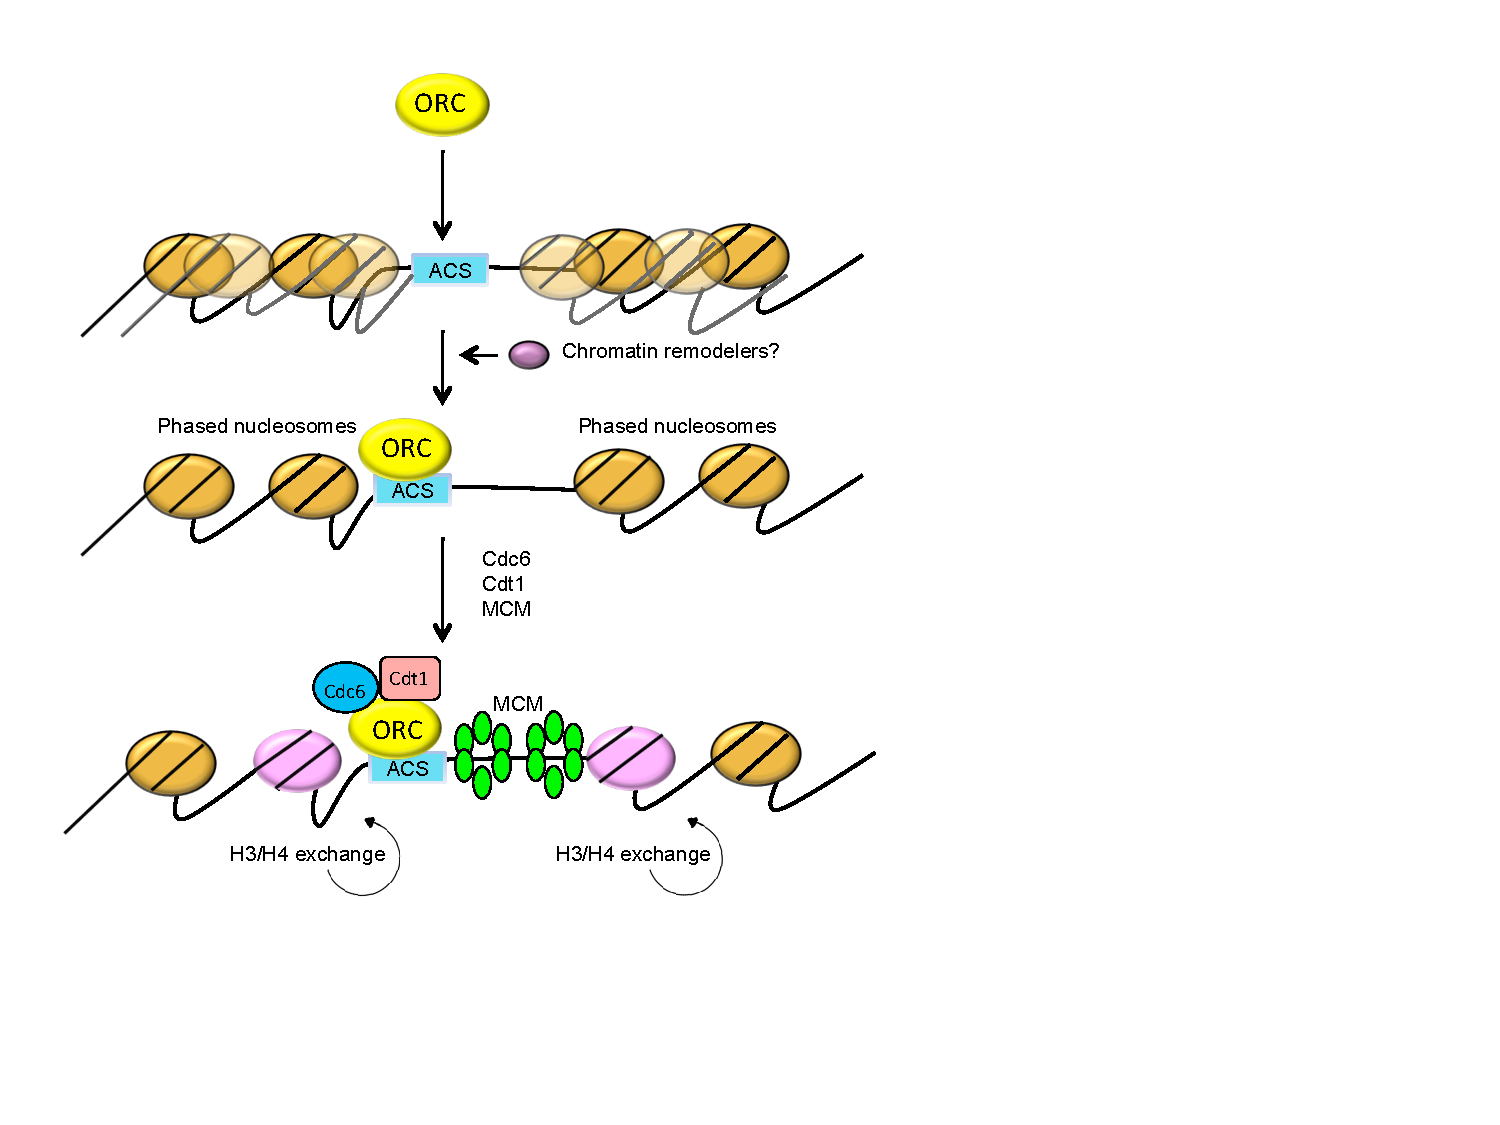
\includegraphics[width=2.5in]{r35_figures/orc_turnover_model.pdf}
%\end{center}
%\vspace{3mm}
%\caption{Pre-RC assembly at replication origins in the context of chromatin. The Mcm2-7 complex is loaded onto origins by ORC, Cdc6 and Cdt1. Nucleosome positioning and chromatin remodeling are conserved features of the eukaryotic DNA replication program\citep{Ding2011-ni}.}%
%\end{floatingfigure}

%In order to duplicate a eukaryotic chromosome within the confines of S-phase, DNA replication must begin at multiple sites along the chromosome.  Failure to completely replicate the chromosomes may result in catastrophic genomic instability\citep{Green2010-ht}.  Origins of DNA replication are defined by conserved trans-acting factors that assemble on the DNA in  a cell cycle regulated manner ({\color{dukeblue}\textbf{Figure 1}}). The origin recognition complex (ORC) functions together with Cdc6 and Cdt1 to load the Mcm2-7 helicase as a double hexamer and form the pre-replicative complex (pre-RC)\citep{Bell2013-pk}. Pre-RC assembly is limited to G1 and serves to `license' the origin for activation in the subsequent S-phase\citep{Siddiqui2013-jz}. As cells enter S-phase, DDK and CDK promote the recruitment of additional proteins to the origin including Cdc45 and the GINS complex to form the pre-initation complex (pre-IC)\citep{Tanaka2013-fl} ultimately resulting in an active helicase complex at each fork.   



%In yeast, DNA replication origins are defined by cis-acting sequence elements that are necessary, but not sufficient, for ORC binding and origin function\citep{Breier2004-tw} suggesting that additional chromatin features modulate origin selection and activation.  In higher eukaryotes ORC exhibits little sequence specificity\citep{Vashee2003-xr} and is preferentially enriched in open and accessible chromatin\citep{MacAlpine2010-ju,Miotto2016-jt}.   We and others have shown that precise nucleosome positioning and active histone exchange are conserved features of ORC binding in yeast\citep{Eaton2010-fq,Berbenetz2010-hh}, \dros\citep{Liu2015-nr,MacAlpine2010-wz} and mammalian cells\citep{Lombrana2013-aw,Lubelsky2011-dj}.  Despite the identification of specific ORC binding sites in higher eukaryotes\citep{Miotto2016-jt}, the mapping of origins has been challenging and controversial\citep{Prioleau2016-bj}.  Recent Okazaki fragment mapping across the human genome identified fewer than a dozen sites were the initiation event could be mapped within 5 kb; instead the vast majority of initiation events mapped to broad zones of 30 kb or more\citep{Petryk2016-rr}.  If ORC localizes to discrete sites of open chromatin marked by DNase I hypersenstivity\citep{MacAlpine2010-ju,Miotto2016-jt}, why are initiation events so dispersed?  One intriguing possibility is that the Mcm2-7 complex may not be restricted to ORC proximal sequences following pre-RC assembly and that the location and density of Mcm2-7 complexes on the chromatin may be responsible for the seemingly stochastic origin activation patterns observed in higher eukaryotes. Alternatively, provocative experiments from the Dutta laboratory  suggest an ORC-independent mode of Mcm2-7 loading in mammalian cancer cells\citep{Shibata2016-uc}. 


%For more than three decades the identification of specific start sites of DNA replication has been a challenge in higher eukaryotes.  Despite the advent of multiple genome-wide approaches for mapping origins, there has only been minimal concordance between different experimental assays including nascent strand abundance assays, ChIP-seq of initiation factors, and mapping replication initiation bubbles.  While some of the disagreement may be due to technical problems, it is becoming increasingly clear that origin selection and activation is a stochastic process in higher eukaryotes.  Recent studies mapping the distribution of Okazaki fragments throughout the genome found fewer than a dozen sites where robust initiation occurred within a 5 kb window, instead the majority of  initiation events mapped to large zones of 30 kb. If ORC localizes to discrete sites of DNase I hypersensitive open chromatin, how and why are the initiation zones so broad?   Recent in vitro work from the Remus lab in \scer demonstrate that the Mcm2-7 complex is able to translocate on the DNA and be pushed away from the site of loading by active transcription.  Experiments from our own laboratory have also demonstrated that active transcription can shape the genomic distribution of the Mcm2-7 complex in \dros.  Thus, a model is emerging whereby ORC loads the helicase complex at ORC binding sites, but that the Mcm2-7 complex is not fixed and is able to translocate along the chromosome.  Alternatively, provocative experiments from the Dutta laboratory may suggest an ORC-independent mode of Mcm2-7 loading in mammalian cancer cells. 

%DNA replication is also the major source of double strand breaks (DSBs) which can occur when the fork encounters nicked DNA or the collapse of a stalled replication fork\citep{Munoz2017-mi}.
%\cite{Halazonetis2008,Hanahan2000,Hanahan2010,Vignard2013}.  
%If not promptly repaired, DSBs may lead to cell death and/or complex chromosomal re-arrangements due to untethered DNA ends\cite{Morgan1998,Hinnen1978}.  
%The factors that mediate DSB recognition and repair via either homologous recombination or non-homologous end joining are molecularly and biochemically well characterized\cite{Symington2011}.
%\cite{Rogakou1999,Vignard2013,Lee2005,Lee2007,Tsukuda2005,Foster2005,Liang2007,Symington2011,Lee2014,Harrison2006,Iacovoni2010,Chai2005,Chai2005a,Burma2001,Burma2001a,Kwon2015,Kwon2014,Geuting2013,Berkovich2007,Sonoda1998,Goldstein2013,Wolner2003,Nakada2003,Shroff2004,Hicks2011,Madabhushi2015,Tsabar2016,Mehta2017,Moore2007,Krogh2004,Kim2007,Alexeev2003,Keogh2006,Costanzo2004,Kurz2004,Haber2016,Haber2012,Avsaroglu2016,Nasmyth1993,Torres-Machorro2015,Celeste2003,Lee2004,Downs2000,Shechter2004,Clapier2009,Morillo-Huesca2010,Lisby2004,Morrison2004,Kimura2006a,Kimura2006,Rothstein1991,Halazonetis2008,Sogo2002,Sugawara2003,Frank-Vaillant2002,Stracker2004,Ataian2006}.
%While nucleosome remodeling and eviction must occur at the break to facilitate strand end-resectioning and Rad51 nucleoprotein filament formation\cite{Renkawitz2014}, it is unclear how the local chromatin architecture at diverse locations throughout the genome impacts the kinetics of DSB induction, recognition and repair.
%\cite{Tsabar2016,Tsukuda2005,Jasin2013}.  

%Finally, a consequence of DNA replication is that chromatin is disassembled ahead of the replication fork; thus, the chromatin, or epigenetic state, needs to be re-established every cell division on the newly synthesized DNA\citep{MacAlpine2013-ds}.   The biochemical mechanisms of chromatin assembly at the replication fork have been well studied \invitro. However, considerably less is known about \invivo kinetics of chromatin assembly, including the association of specific transcription factors and re-establishment of nucleosome positioning behind the replication fork.  



%Stalled DNA replication forks may lead to double strand breaks (DSBs) 
%The local chromat

%F31
%Elegant genetic and biochemical experiments have elucidated many of the molecular events associated with the recognition and repair of  double strand breaks.  In addition to the factors required for break recognition, processing and repair via homologous recombination or non-homologous end joining, the local chromatin environment also influences the accessibility of the break site and the kinetics recognition and repair.  Further there are also global changes in epigenetic state and nuclear architecture that occur in a cell burdened with DSBs.   Prior experiments have identified loss of nucleosome occupancy and [specific remodeling? events] at the MAT locus; however, they have lacked the temporal and spatial resolution to discern the mechansim by which which nucleosome occupancy is lost (eg. eviction or sliding?).   In addition, it is unclear how dependent the observed changes in nucleosome occupancy are on the local chromatin structure and state of the MAT locus. 


%This model may also address provactive experiments from the Dutta laboratory suggesting that ORC is not essential for replication in mammalian cancer cells.  Either there are indpendent Mcm2-7 loading mechnanisms, or that there is some minimal ORC in the mutants (estimated to be less than 1\%) capacity that is sufficient for loading the Mcm2-7 complex. 

%image of stochastic origin selection. -- where am i going with this.

%Until recently, origin selection was thought to be dependent on ORC binding.  However, 

%Although we have begun to elucidate the chromatin determinants of o

%In addition to conserved trans-acting factors, origins of DNA replication are also defined by cis-acting sequences and  chromatin features.  In \scer, a degenerate T-rich sequence, termed the ACS (ars consensus sequence) is necessary, but not sufficient for ORC binding and origin function. However, in higher eukaryotes, ORC exhibits little sequence specificity and is preferentially enriched in open and accessible chromatin \cite{macalpine,struhl}. 

 


%with active and repressive chromatin states contributing to

%-- not surpring regulated origin activity. [also cite oscar]

%correlations individual origins

%finally -- chromatin assembly


%Chromatin faciltates the packaging and compaction of the genome and

%how to get back to replication. 

%Origin selection is not a stochastic process -- 

%Origin selection and activation are shaped by the chromatin environment and nuclear architecture.  

%In addition to conserved trans-acting factors, origins of DNA replication are also defined by cis-acting sequences and epigenetic features.  


%Overview figure
 %   nucleosome dynamics origin activation
  %  chromatin assemblyOr
   % mcm redistribution and origin activation
    %transcription
    %DNA breaks
    


%In contrast, the cis-acting sequence elements that contribute to origin function are less understood.  In \scer\ , the ACS (ARS consensus sequence) is a degenerate T-rich sequence that is necessary, but not sufficient, for ORC binding and origin function\citep{BCC04}. In addition, other poorly defined sequence elements (termed B-elements) also contribute to origin function\citep{Marahrens:1992zr}. However, in metazoan systems, ORC exhibits little if any sequence specificity \invitro\citep{VCL+03,RBB04}, suggesting that other chromosomal features (e.g. chromatin accessibility, histone modifications, transcription factors, etc) may participate in origin selection. Indeed, we and others have shown that nucleosome organization and active histone exchange are conserved features of ORC localization in \scer\citep{EGK+10} and \dros\citep{MGP+10,modENCODE-Consortium:2010vn,Eaton:2011ys}.  

%Our research program is focused on understanding how the local chromatin environment impacts the DNA replication program to maintain both genetic and epigenetic inheritance. 

%Atouble hexamer of the Mcm2-7 complex is loaded.  

%notes for donald
%Letters of Support:  The application must include a letter from the institution’s Authorized Organizational Representative (AOR) indicating that they are aware of and accept the condition that other NIGMS research awards must be relinquished and pending NIGMS research applications, except as allowed in Section I, withdrawn as a condition of receiving a MIRA, and providing a statement that if chosen to receive an award, the PD/PI will devote at least 51% of his/her time available for research to this award. The time available for research should be determined in person-months and should not include time expended toward teaching, administration, and/or clinical duties.

%cost share of 26%

%begin to assemble on the DNA in G1 of the cell cycle.

%In addition to conserved trans-acting factors, origins of DNA replication are also defined by cis-acting sequences and epigenetic features.  

%need to mention dutta paper
%hyrien paper and 


%The trans-acting factors taht


%DNA replication  assays 

%DNA replication --> huge progress
%chromatin and origin selection regulation larger view nuclear and chromatin.  We
%yeast vs rest of eukaryotic systems
%chromatin assembly
%Transcription
%DNA Damage




%Genetic and epigenetic inheritance

%Figure


%It is essential that the genome be replicated accurately and completely within the confines of S-phase. Failure to completely replicate the chromosomes may result in catastrophic genomic instability\citep{GFL10}. Replication initiates from multiple sites, termed origins of replication, along each chromosome. In metazoans, DNA replication is a dynamic process capable of responding to changes in the developmental program\citep{HMM95}. Increasing evidence suggests that the DNA replication program is regulated, in part, by the organization and accessibility of the local chromatin environment\citep{Berbenetz:2010vn,EGK+10,DHH10}. Currently, very little is known about how the architecture and dynamics of the local chromatin environment modulate the DNA replication program to maintain genomic stability.


%In all eukaryotes origin selection is mediated by the formation of a multi-protein complex, called the pre-replicative complex (pre-RC), on DNA during G1 of the cell cycle\citep{BD02}({\bf \color{dukeblue}Figure 1}). Potential origins of replication are marked by the origin recognition complex (ORC). ORC together with Cdc6p and Cdt1p cooperate to load the Mcm2-7 helicase forming the pre-RC in G1\citep{MLB06,BS08}. The pre-RC functions as an essential initiator complex, and its components are conserved in all eukaryotes. The formation of the pre-RC in G1 on the DNA in effect licenses that sequence to function as an origin of replication during the subsequent S-phase\citep{Dif04}.

%In contrast, the cis-acting sequence elements that contribute to origin function are less understood.  In \scer\ , the ACS (ARS consensus sequence) is a degenerate T-rich sequence that is necessary, but not sufficient, for ORC binding and origin function\citep{BCC04}. In addition, other poorly defined sequence elements (termed B-elements) also contribute to origin function\citep{Marahrens:1992zr}. However, in metazoan systems, ORC exhibits little if any sequence specificity \invitro\citep{VCL+03,RBB04}, suggesting that other chromosomal features (e.g. chromatin accessibility, histone modifications, transcription factors, etc) may participate in origin selection. Indeed, we and others have shown that nucleosome organization and active histone exchange are conserved features of ORC localization in \scer\citep{EGK+10} and \dros\citep{MGP+10,modENCODE-Consortium:2010vn,Eaton:2011ys}.  Our research program is focused on understanding how the local chromatin environment impacts the DNA replication program to maintain both genetic and epigenetic inheritance.  

%A mechanistic understanding of how origins are established and regulated in proliferative cells will have far-ranging implications for developmental, stem cell, and cancer biology. Failure to completely duplicate the genome {\em exactly} once per cell cycle in mitotic cells results in genomic instability\citep{GFL10} -- a hallmark of cancer. Two pre-RC components, Cdc6p\citep{GKD+06} and Cdt1p\citep{AFS+02}, have oncogenic potential, presumably mediated by re-replication induced genomic instability which can include gene amplification\citep{GFL10}. Conversely, a decrease in replication initiation (as in the {\em MCM4} ({\em chaos3}) mutant in mouse) also leads to chromosomal breaks, genome instability and cancer\citep{SAL+07}. Finally, recent studies have linked mutations in multiple components of the pre-RC (including ORC) to Meier-Gorlin syndrome, an autosomal recessive form ofdwarfism\citep{Bicknell:2011ys,Bicknell:2011zr}. Only by identifying and characterizing the specific chromosomal elements that direct and regulate DNA replication will we be able to understand how these processes are established and maintained to preserve the expression and inheritance of genetic information. 
%\section{Recent Research Progress}
\sheading{Chromatin organization and DNA replication in \scer}
\ssheading{Chromatin architecture of replication origins}
To better understand how the chromatin environment impacts the selection and regulation of replication origins, we evaluated the DNA occupancy of nucleosomes and the majority of DNA-binding proteins (\eg transcription factors and replication initiation proteins) to generate genome-wide chromatin occupancy profiles (GCOPs)({\color{dukeblue}\textbf{Figure 2}}). Briefly, total chromatin is digested with micrococcal nuclease (MNase) and all of the recovered DNA fragments are subjected to paired-end next-generation sequencing\citep{Belsky2015-li,Henikoff2011-vo}.  Importantly, the size of the sequenced fragment represents whether it was protected by a nucleosome ($\sim$147 bp) or a DNA-binding factor ($<$50 bp). This assay is factor agnostic and reveals specific footprints for more than 70\% of the yeast DNA-binding factors\citep{Henikoff2011-vo}.  Although, the assay only provides information about the occupancy state of the DNA, we can often infer the identity of the factor bound from motifs and prior genomic experiments.  
\begin{floatingfigure}[lt]{2.8in}
\vspace{-8mm}
\begin{center}
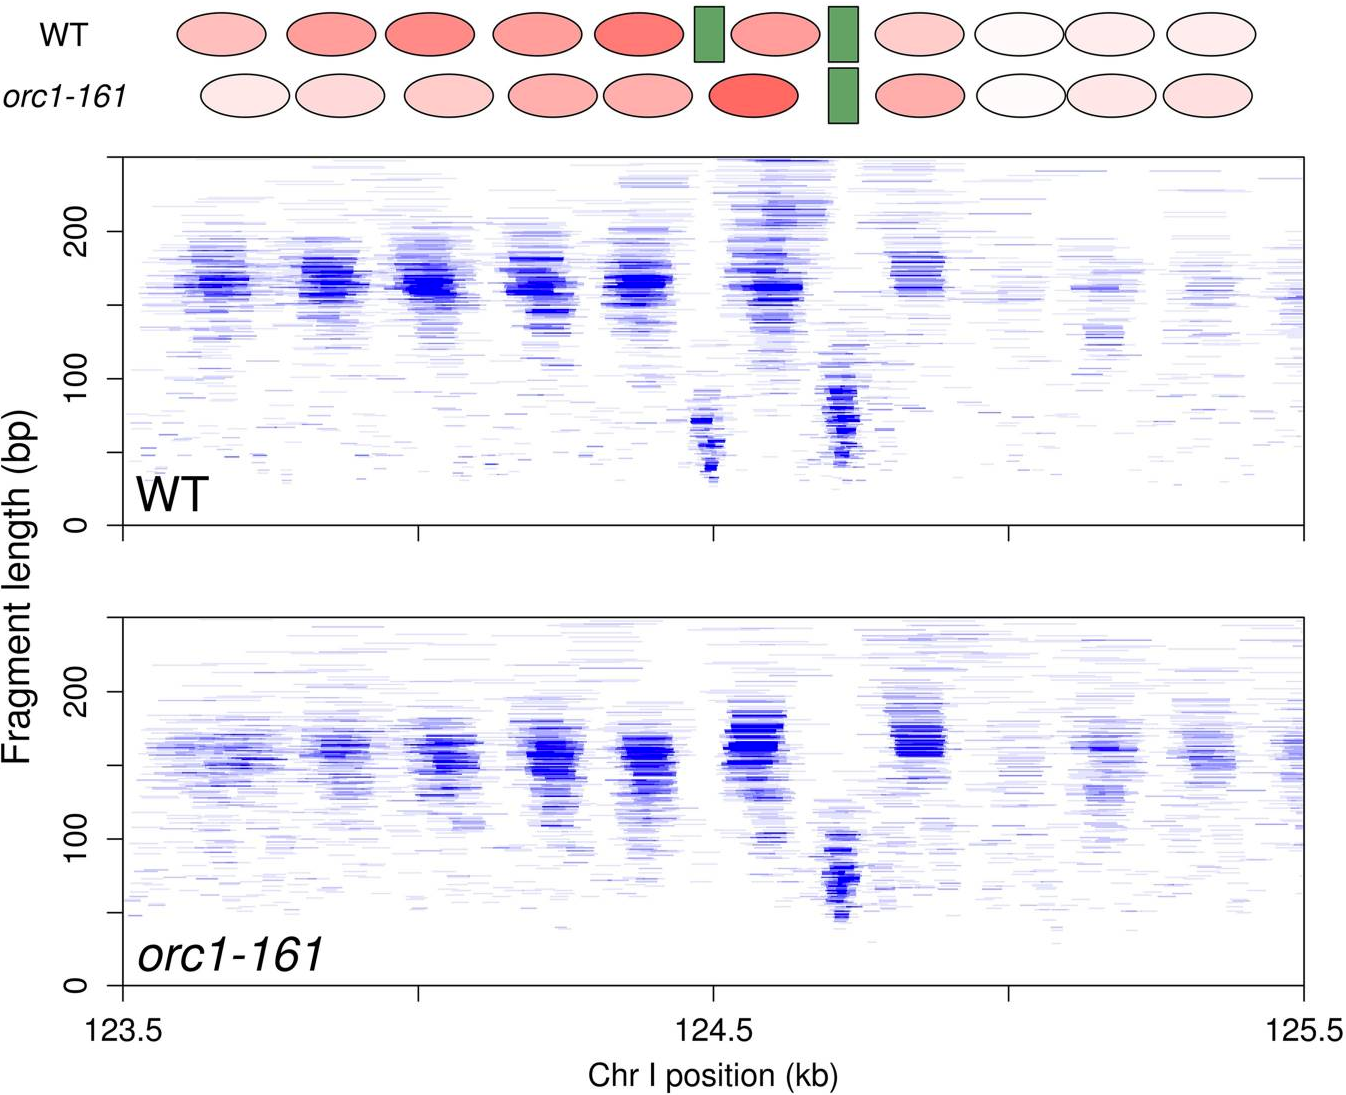
\includegraphics[width=2.8in]{r35_figures/orc_chromatin_gcop.png}
\end{center}
\vspace{3mm}
\caption{GCOP of a replication origin.  MNase protected DNA fragments were subjected to paired-end sequencing and the resulting fragment lengths were plotted as a function of chromosomal position.  Well phased fragments at $\sim$150 bp represent sequences protected by nucleosomes (red ovals in cartoon) and smaller fragments represent other DNA binding factors (\eg ORC at the ACS and Abf1).  In an \textit{ORC1-161} mutant the footprint at the ACS disappears at the non-permissive temperature.}%
\end{floatingfigure}%
Our `footprinting' of the \scer genome at distinct cell cycle stages provided the  %the We `footprinted' the \scer\ genome at multiple points in the cell cycle including G2 (ORC alone) and G1 (pre-RC assembly)\citep{Belsky2015-li}.  Together, these experiments provide the 
following advances and new insights into our understanding of the DNA replication program: i) a novel method to map origins of DNA replication by their ORC-dependent chromatin footprints -- this data provides structural information not only about ORC binding but also the surrounding chromatin and adjacent DNA binding factors at each individual origin; ii) identification of a non-canonical class of inefficient origins that lacked an ORC-dependent footprint in G2, but exhibited a clear footprint in G1 -- the mechanistic implication being that determinants of replication efficiency are established in G2 prior to pre-RC assembly; iii) nucleosome remodeling at the origin is required for efficient origin activation, but not pre-RC assembly -- highlighting the importance of nucleosome dynamics for downstream initiation events including origin unwinding and activation; iv) the loading of a singe Mcm2-7 double hexamer per origin in complex with either the up or downstream flanking nucleosome -- addressing a fundamental question in the field -- where, in relation to ORC, and how many Mcm2-7 double-hexamers are loaded per origin \invivo. 

Recent work has sought to identify the chromatin remodeling activities responsible for nucleosome dynamics at replication origins.  %We have systematically evaluated all single, double and triple combinations of non-essential chromatin ATP-dependent chromatin remodelers in \scer for their impact on ORC binding, pre-RC assembly and origin activity. While the replication program was surprisingly resistant to loss of ATP-dependent chromatin remodelers, 
We found that both \textit{ISW1} and \textit{CHD1} activity are required for origin activation of inefficient origins (manuscript submitted). In collaboration with Steve Bell, we have recently demonstrated that the \invitro assembly of nucleosomes by specific chromatin remodeling enzymes can impact pre-RC assembly and initiation in a reconstituted system\citep{Azmi2017-gg}.

\sheading{Establishment of the replication program and maintenance of genome integrity in \dros}
As a data production center for the model organism ENCODE (modENCODE) project we generated more than one hundred genome-wide datasets describing the \dros replication program\citep{Mod_Encode_Consortium2010-io}.  In the capstone manuscript for the modENCODE project, more than 1400 genomic datasets from modENCODE and ENCODE revealed conserved principles and features of chromatin organization between flies, worms and humans\citep{Ho2014-xa}. %We identified conserved features of chromatin state and genome organization that were linked to the establishment of the DNA replication program. 
%In addition to the capstone manuscript, we published 12 manuscripts over the course of the project. 
Below I've highlighted several of our mechanistic follow-up studies in \dros that were supported by our NIGMS R01.

\ssheading{DNA replication and transcription programs respond to the same epigenetic cues}
%The a time at which a sequence replicates during S-phase has long been coordinated with transcriptional activity in higher eukaryotes. 
We and others have correlated gene expression, open chromatin and chromatin modifications with origin location and replication timing data.  However, correlation does not  imply causation and due to multiple activating and repressive chromatin modifications it has been difficult to mechanistically assign a direct role to specific chromatin modifications in regulating the DNA replication program. We demonstrated that the early replication of the \dros male X chromosome was dependent on dosage compensation and the male-specific H4K16 hyperacetylation of the X chromosome\citep{Lubelsky2014-zn}.  These results demonstrate that the transcription and DNA replication programs respond to the same epigenetic cues.

\ssheading{H4K20 monomethylation and genome integrity}
PR-Set7 is a cell cycle regulated methyl transferase that specifically monomethylates H4K20\citep{Beck2012-uc}.  In mammalian cells, loss of PR-Set7 and the resulting H4K20me1 is associated with delayed S-phase progression and elevated DNA damage presumably due to defects in pre-RC assembly and origin activation\citep{Tardat2010-qc}.  %However, prior studies only examined a handful of mammalian origins and it remained possible that the observed origin specific phenotypes were not due to perturbation of histone methylation, but PR-Set7 mediated methylation of other cell cycle  factors\citep{Shi2007-gz}. 
Although PR-Set7 is an essential gene in \dros, alanine substitution histone tail mutants (H4K20A) were sick but viable\citep{McKay2015-nn}, arguing that H4K20 methylation is not essential for DNA replication. We found that deregulation of PR-Set7 activity did not impact origin activation in \dros, but rather H4K20 mono-methylation was required for maintaining genomic integrity of late replicating domains\citep{Li2016-fi}.  We propose that the accumulation of unmodified H4K20 hinders fork progression through late replicating sequences and results in stochastic replication fork collapse.


\ssheading{Mcm2-7 Paradox}
The `MCM Paradox' describes a %long standing 
series of %seemingly
paradoxical observations regarding the quantity and location of the Mcm2-7 helicase complex during S-phase in higher eukaryotes\citep{Takahashi2005-bz}. Briefly, there is a vast excess of the Mcm2-7 complexes relative to origins of replication or ORC binding sites, the majority of which are %; %the Mcm2-7 complexes do not appear to localize to ORC by immunofluorescence experiments
%and the vast majority of the Mcm2-7 complex are 
dispensable during an unperturbed S-phase. We examined the `MCM Paradox'  using  genomic and biochemical approaches  to understand the mechanisms by which excess Mcm2-7 are loaded and distributed throughout the genome to preserve genomic integrity\citep{Powell2015-af}.  We found that during G1, Mcm2-7 is loaded onto chromatin in two distinct phases -- both of which rely on the canonical pre-RC assembly pathway including Dup/Cdt1 and Cdc6.  In the first phase of pre-RC assembly, a minimal level of Mcm2-7 is loaded specifically at ORC binding sites throughout the genome in a CDK independent manner.  There is also a second wave of pre-RC assembly that is CDK dependent which is required for the loading of the full complement (40 fold increase) of Mcm2-7 onto chromatin.  Strikingly, the full complement of Mcm2-7 is not restricted to sequences immediately adjacent to ORC binding sites, but rather distributed throughout the genome and shaped by active transcription.  %We find that the full complement of Mcm2-7 complex is displaced from actively transcribed regions suggesting that transcription can push or displace the Mcm2-7 complex through gene bodies.  
%Recent work from the Remus laboratory in \scer  has demonstrated that the Mcm2-7 complex can be pushed away from ORC binding sites by RNA Polymerase \invitro and \invivo resulting in origin activation being displaced from the site of pre-RC assembly\citep{Gros2015-oo}.  Together, 
These data provide an intriguing model whereby the transcription program may shape the distribution of the Mcm2-7 complex and ultimately origin location which may explain the seemingly random distribution of metazoan origins in higher eukaryotes\citep{Petryk2016-rr}.


%\section{Overview of Future Research}
%All DNA-templated processes in the nucleus occur in the context of the local chromatin environment.  
My research program has been focused on understanding how chromatin shapes the DNA replication program in \scer and \dros. We have taken advantage of the unique features and strengths of each organism -- well defined cis-acting and chromatin determinants of origin function in \scer and the more complex epigenetic features that regulate origin selection and activation in \dros.  
We will continue to use the strengths of each model system to address fundamental questions regarding the inheritance of genetic and epigenetic information. We are also excited to extend our nucleotide resolution GCOPs to investigate chromatin dynamics associated with DNA damage and repair. Finally, in collaboration with Alex Hartemink (Computer Science, Duke) and Greg Crawford (Pediatrics, Duke) we have recently been awarded a collaborative NIGMS R01 to probe chromatin-based mechanisms inside the `black box' of transcriptional regulation. 

\sheading{DNA Replication}
\ssheading{Chromatin dynamics during initiation of DNA replication in \scer}
%Beginning in G1, a series of tightly orchestrated biochemical events occur at each origin of DNA replication ultimately leading up to initiation of DNA replication in S-phase\citep{}.  
How does the local chromatin environment, which is unique to each origin, modulate ORC binding, pre-RC assembly, and initiation?  We have already identified a series of specific nucleosome remodeling events that occur during ORC binding (G2)\citep{Eaton2010-fq} and pre-RC assembly (G1)\citep{Belsky2015-li} which are correlated with origin efficiency\citep{Belsky2015-li}. We now propose to examine changes in chromatin structure that are associated with the assembly of the pre-initiation complex and priming of DNA replication.  We hypothesize that the steps leading up to unwinding of the DNA and the transition of the Mcm2-7 complex from encircling dsDNA to ssDNA will result in the specific eviction or sliding of origin flanking nucleosomes.  We also expect that local chromatin features unique to each origin (\eg flanking DNA binding factors and local transcription) will contribute to the symmetry and extent of nucleosome remodeling and eviction.  We will use conditional  mutants (ts, degron, anchor away\citep{Haruki2008-qe} or combinations) of key initiation factors (\eg primase or \textit{Mcm10}) to block DNA replication immediately prior to initiation.  Alternatively, we will attempt to block initiation using the conditional expression of MCM mutants (MCM3RA) defective for initiation but not Cdc45 and GINS loading \invitro\citep{Kang2014-iu}. While the GCOP mapping will provide a factor agnostic assessment of origin chromatin architecture, we will also use ChIP-exo\citep{Rhee2011-yi} to probe the location and identity of specific structural footprints observed in the GCOPs.  We expect to identify and decipher the key changes in chromatin structure that accompany the transition of the pre-RC into the pre-IC and ultimately into a functional bidirectional replisome.  
%\ssheading{Mcm2-7 loading is limited by chromatin architecture}
\begin{floatingfigure}[r]{2.0in}
\vspace{-8mm}
\begin{center}
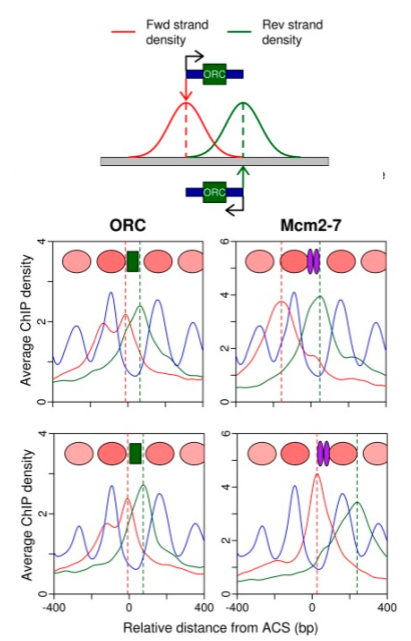
\includegraphics[width=2.0in]{r35_figures/mcm_histone.png}
\end{center}
\vspace{3mm}
\caption{Asymmetric Mcm2-7 loading at origins.  The ends of ChIP fragments (red,green) were analyzed to precisely localize ORC and MCM2-7 relative to nucleosomes (blue).  ORC resolves to the ACS and exhibits an interaction with the leftmost flanking nucleosome.  Mcm2-7 localizes up or downstream of the ACS and is in complex with the up or downstream flanking nucleosome.}%
\end{floatingfigure}%


Bi-directional DNA replication emanating from an origin is an inherently symmetrical event.  Despite this symmetry, there is striking asymmetry in a number of origin features.  For example, the T-rich ACS and downstream A-rich region constitute a polar sequence that is asymmetrically located between two flanking nucleosomes. Further, we have demonstrated that the loading of double hexamer of Mcm2-7 occurs either up or downstream from the oriented ACS and is tightly coupled with the flanking nucleosome ({\color{dukeblue}\textbf{Figure 2}}) \citep{Belsky2015-li}. We will identify the mechanism(s) by which Mcm2-7 loading is asymmetric, coupled with a flanking nucleosome, and limited to one double hexamer per origin.  Although the significance of why each origin adopts a specific Mcm2-7 loading configuration (up or downstream of the ACS) is currently unclear, it is reasonable to speculate that specific configurations may facilitate initiation and origin efficiency -- especially in the context of other surrounding chromatin features such as histone modifications, direction of transcription and nucleosome turn-over.  We will first test the role of known and conserved mutants that disrupt the interaction between Mcm2 and histone H3\citep{Huang2015-fk,Foltman2013-dk}.  While these Mcm2 mutations do not exhibit a gross defect in transit through S-phase, they are thought to impair chromatin assembly and disassembly at the fork\citep{Foltman2013-dk}.  If we observe that interaction with the origin flanking nucleosome is disrupted or there is loss of polarity in Mcm2-7 loading, we will carefully assess replication timing and the kinetics of initiation \invivo.  Alternative approaches will include a proteomic based approach to identify potential histone modifications that are enriched on nucleosomes immunoprecipiated with the Mcm2-7 complex (LoS Moseley), and disrupting transcription of origin flanking genes to prevent transcription into the origin which may influence the polarity of origin loading\citep{Gros2015-oo}.  Importantly, does elimination of any of these mechanisms result in the loading of additional Mcm2-7 double hexamers per origin or perturbations in origin efficiency? Finally, we will continue to collaborate with the Bell laboratory in order to confirm and further dissect our \invivo findings in a reconstituted system (LoS Bell).  

\ssheading{Origin selection and activation in \dros}
Despite the conservation of replication initiation factors, identifying the precise locations where DNA replication starts in higher eukaryotes has been a long standing and controversial question\citep{Prioleau2016-bj}. The canonical model is that ORC recruits the Mcm2-7 helicase to specific locations in the genome to function as origins in the next S-phase. Although ORC does map to specific sites in the genome\citep{Miotto2016-jt}, initiation of DNA replication is not confined to specific locations but instead maps to broad zones of initiation ($>$30 kb)\citep{Petryk2016-rr}. We propose that initiation in higher eukaryotes is dependent not on the localization of ORC, but rather the genome-wide distribution of the Mcm2-7 complex. This model is supported by our recent work demonstrating that the distribution of the Mcm2-7 complex as \dros cells enter S-phase is not associated with ORC, but rather distributed throughout the genome and shaped by transcription\citep{Powell2015-af}.  These data are also supported by \invitro and \invivo studies in yeast where the precise location of the Mcm2-7 complex can be displaced for short distances away from the origin by active transcription\citep{Gros2015-oo}.  

The loaded Mcm2-7 complex is capable of translocating on naked DNA -- but how does the complex seemingly redistribute throughout the complex chromatin landscape of a metazoan chromosome?  Three possible models are that the Mcm2-7 complex is able to i) translocate away from the ORC binding site; ii) be loaded at a distance from the ORC binding via DNA looping; iii) load promiscuously throughout the genome in an ORC independent manner\citep{Shibata2016-uc}.  The genomic tools and cell cycle synchronization methods that we developed to examine the CDK-regulated step wise loading of the Mcm2-7 complex in \dros coupled with recent advances in CRISPR/Cas9 methodologies\citep{Kunzelmann2016-sf} have us well positioned to test these models.  For example, while we have shown loading of the full Mcm2-7 complement is dependent on Cdc6 and Cdt1\citep{Powell2015-af}, we can also conditionally remove ORC (using degrons) prior to the second wave of Mcm2-7 loading to test the dependence on ORC.  These and other experiments will provide new insights into how metazoan origins of replication are specified.   

We will continue our ongoing collaboration with the Duronio group at UNC to investigate the role of specific chromatin marks in regulating replication timing, genome stability and origin usage in \dros\citep{Li2016-fi}(LoS Duronio). Using a genetic histone replacement strategy\citep{McKay2015-nn}, we will be able to directly test the impact of specific histone tail mutants on DNA replication in proliferating tissues. %Importanty, this approach provides a direct assesment of the role of specific    %The Duronio group has developed a genetic histone replacement strategy for the fly\citep{McKay2015-nn}, allowing us to directly test the impact of specific histone tail mutants on DNA replication in proliferating tissues (\eg imaginal discs).  Unlike manipulation of chromatin modifying enzymes, this approach eliminates potential off target actions and provides an unbiased assessment of the role of specific chromatin modifications in regulating the DNA replication program.
\begin{floatingfigure}[l]{3.55in}
\vspace{-6mm}
\begin{center}
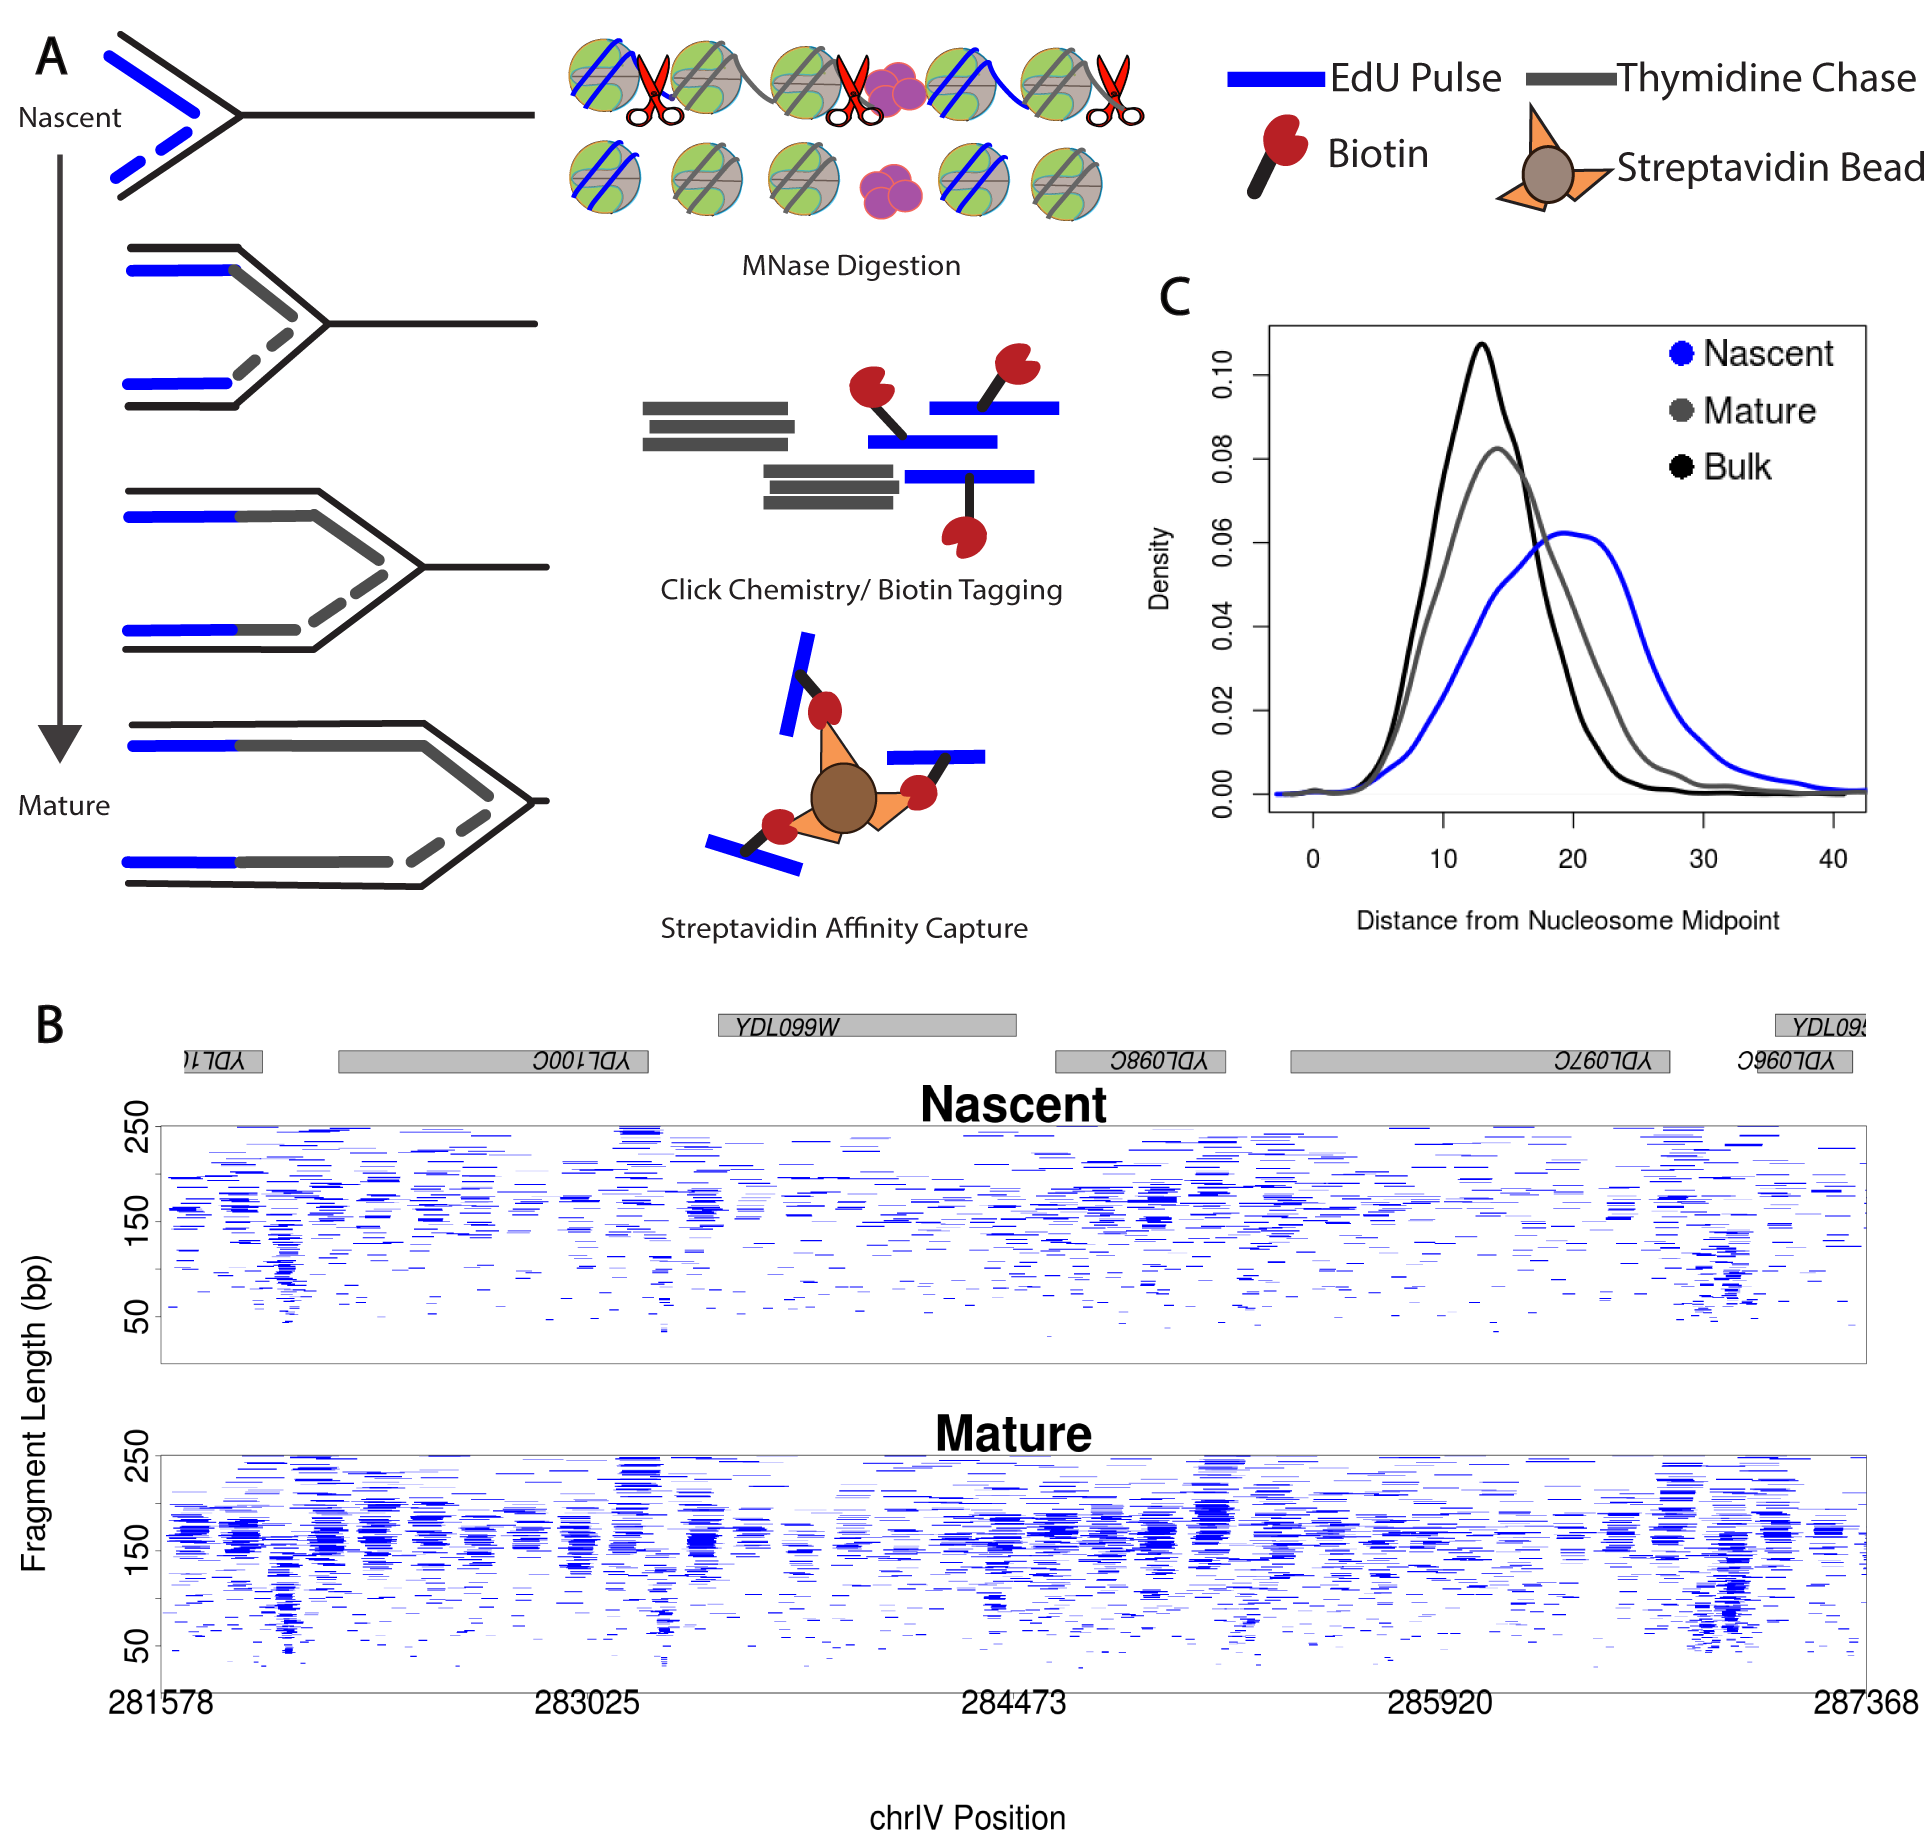
\includegraphics[width=3.55in]{r35_figures/dave_figure2.png}
\end{center}
\vspace{2mm}
\caption{\textbf{A}. Schematic for determining chromatin structure for nascent and maturing chromatin labeled with EdU. \textbf{B}. GCOP of nascent and mature chromatin. \textbf{C}.  Distribution of nucleosome midpoints for bulk (black), mature (gray) and nascent (blue) chromatin demonstrating that nascent chromatin lacks precise nucleosome positioning.}%
\end{floatingfigure}


%\ssheading{Chromatin assembly behind the replication fork}
\ssheading{Role of DNA Replication in Establishing Chromatin Architecture}
%DNA replication plays an integral role in propagating the parental epigenetic state to newly copied sequences.  
DNA replication results in the complete disassembly of chromatin, which must be re-established behind the replication fork in order to propagate the original epigenetic state. Chromatin restoration on nascent DNA is a complex and regulated process, including nucleosome assembly, remodeling, and deposition of histone variants\citep{MacAlpine2013-ds}.  Recently, proteomic techniques have been developed to study the proteins associated with replicative chromatin in a temporal fashion\citep{Alabert2014-io,Sirbu2011-wx}. %Nascent and mature chromatin are differentiated by the incorporation of nucleoside analogs (e.g. BrdU, EdU) followed by the immunoprecipitation of labeled chromatin after a short pulse of only a few minutes for nascent chromatin or followed by a longer chase period for mature chromatin. 
While these approaches focus on studying large pools of proteins associated at multiple phases of replication, they do not provide the spatial or temporal information of chromatin maturation at individual loci. 

We have extended our GCOP assay to profile EdU labeled chromatin in order to examine chromatin occupancy for nascent and mature chromatin ({\color{dukeblue}\textbf{Figure 3}}).  Similar approaches to examine chromatin maturation have very recently been reported in yeast\citep{Vasseur2016-rx} and \dros\citep{Ramachandran2016-zu}; however, these approaches focused on nucleosomes and not the occupancy of smaller DNA binding proteins.  As a proof of principle, we pulse labeled asynchronous cells with EdU for 10 minutes and chased with thymidine for 0 or 40 minutes to recover nascent and mature chromatin, respectively.  Importantly, the  assay monitors the kinetics of chromatin maturation behind the fork. We find significantly less chromatin organization in the nascent chromatin relative to mature chromatin. %Interestingly, we also find locus specific differences in chromatin maturation dependent on origin efficiency.  The chromatin structure at efficient origins matures faster than inefficient origins suggesting there are differences in origin re-assembly between actively firing and passively replicated origins.

We expect to address multiple fundamental questions in chromatin biology. For example, are there locus-specific differences in chromatin maturation? -- perhaps we will identify `epigenetic fragile sites' or locations that are slow to re-establish their chromatin landscape. Is there a difference in replication or transcription dependent chromatin organization? Do all DNA-binding factors re-associate with the chromatin with the same kinetics, or are there factor-specific and locus specific differences?   As this work matures we will interrogate the role of histone chaperones and chromatin remodelers in the re-establishment of chromatin organization behind the replication fork.  

%\newpage
\sheading{DNA Damage}
Elegant genetic and biochemical experiments have elucidated many of the molecular events associated with the recognition and repair of  double-strand breaks\citep{Haber2016-ca,Lieber2010-cl,Renkawitz2014-jz,Jasin2013-fv}.  In addition to the factors required for break recognition, processing and repair via homologous recombination or non-homologous end joining, the local chromatin environment also influences the accessibility of the break site
and the kinetics of recognition and repair\citep{Price2013-lp,Smerdon1991-sv}. Prior studies have noticed a loss of nucleosome occupancy following break recognition by the Mre11-Rad50-Xrs2 (MRX) complex\citep{Tsukuda2005-bm}, which is a conserved phenomena in mammalian cells\citep{Berkovich2007-it,Goldstein2013-kb}. However, these experiments have lacked the temporal and spatial resolution to discern the precise mechanisms by which nucleosome organization and occupancy are lost (\eg eviction or sliding of nucleosomes?) and the fate of bound transcription factors.  We will use our GCOP assay to precisely and quantitatively profile the temporal cascade of chromatin structure changes that occur surrounding site-specific double strand breaks and their subsequent repair via NHEJ or HR. Our investigations into DNA damage and DSB repair will be further augmented by a collaboration with Jim Haber at Brandeis (LoS Haber). %In order to interpret our GCOP data in the context of the DNA repair field, we will received guidance and advice from Jim Haber at Brandies (LoS Haber).


\ssheading{Chromatin alterations at site specific DSBs}
%using a donorless
We are able to monitor the specific chromatin changes that occur in response to a GAL::HO induced DSB in the absence of a donor for HR mediated repair.  Proof of principle experiments at an ectopic HO cut site in the \textit{PHO5} locus reveal the asymmetric eviction of a flanking nucleosome, sliding of distal nucleosomes until impeded by a neighboring Fkh2 bound site and the recruitment of a DNA binding factor to the break ({\color{dukeblue}\textbf{Figure 4}}).  Although we can detect a new occupancy footprint at either side of the  break, we do not know the identity of the factor -- it could represent the MRX complex, Ku proteins, or even HO endonuclease itself. Importantly, the wealth of existing molecular and genetic data regarding trans-acting factors involved in double-strand break recognition and repair %, coupled with the `awesome power of yeast genetics', 
will enable us to undertake a %systematic
candidate based approach to identify the responsible factor(s). In a single GAL::HO strain, we have used markerless CRISPR/Cas9\citep{Anand2017-dp} to introduce multiple ectopic HO-endonuclease recognition sequences at loci with distinct chromatin states (TF bound regions, centromeres, telomeres, origins, etc.). By simultaneously interrogating the site specific chromatin changes that occur across a broad survey of different ectopic locations for the break, we will begin to be able to identify the rules by which the local chromatin structure influences DSB recognition and the kinetics of repair.
\begin{floatingfigure}[r]{2.5in}
\vspace{-4mm}
\begin{center}
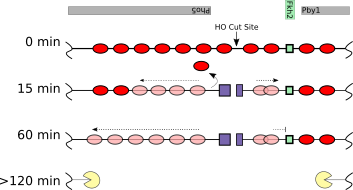
\includegraphics[width=2.5in]{r35_figures/cut_process.png}
\end{center}
\vspace{4mm}
\caption{DSB at the \textit{PHO5} locus. GCOP summary of the temporal dynamics of chromatin alterations immediately following a GAL::HO induced DSB at the \textit{PHO5} locus. }%
\end{floatingfigure}


%In collaboration with the Haber laboratory (Haber letter) we have used markerless CRISPR/Cas9\cite{Dekker2017} to introduce multiple ectopic HO-endonuclease recognition sequences into six loci with distinct chromatin states (TF bound regions, centromeres, telomeres, etc.) in a single GAL::HO yeast strain.  %Site specific DSBs at these ectopic loci is rapid and dependent on GAL::HO induction.% and is rapid with 90\% of the DNA being cut within 15-30 minutes of galactose addition.  
%We are able to %simultaneously 
%to comprehensively, and in a factor agnostic manner, 
%monitor the specific chromatin changes that occur in response to a DSB over time in the absence of a donor template for repair.  Proof of principle experiments at the \textit{PHO5} locus reveal the asymmetric eviction of a flanking nucleosome, sliding of distal nucleosomes until impeded by a neighboring Fkh2 bound site and the recruitment of a DNA binding factor to the break ({\color{dukeblue}\textbf{Figure 5}}).  Although we can detect a new occupancy footprint at either side of the  break, we do not know the identity of the factor -- it could represent the MRX complex, Ku proteins, or even HO endonuclease itself. Importantly, the wealth of existing molecular and genetic data regarding trans-acting factors involved in double strand break recognition and repair %, coupled with the `awesome power of yeast genetics', 
%will enable us to undertake a %systematic
%candidate based approach to identify the responsible factor(s).  By simultaneously interrogating the site specific chromatin changes that occur across a broad survey of different ectopic locations for the break, we will begin to be able to identify the rules by which the local chromatin structure influences DSB recognition and the kinetics of repair.



\ssheading{Interrogating chromatin structure following repair}
%Repair of the DNA break may occur through either HR via a homologous donor template or NHEJ.  
We are interested in understanding how epigenetic information is restored following repair of the break. %Although prior experiments have clearly shown a loss of nucleosome occupancy surrounding the break at the MAT locus and in mammalian cells, these have all lacked the precision to observe subtle changes in chromatin organization and are often confounded by strand resectioning.
For example, at \textit{PHO5} immediately following a break we observe eviction of a flanking nucleosome as well as more distal nucleosomes sliding away from the break -- 
if we turn off HO-endonuclease and 
allow the cells to proceed through repair by NHEJ in the absence of a donor template %or in a \textit{rad51} mutant 
does the resulting chromatin recapitulate the organization prior to the break? Although prior experiments have shown that both replication independent and dependent chromatin assembly mechanisms contribute to restoring nucleosome occupancy\citep{Li2016-wg}
%\citep{Tsabar2015,Li2016} 
they have lacked the resolution to precisely and quantitatively describe nucleosome occupancy and the re-association of TFs.
% or were conducted at the \textit{MAT} locus which has inherently poorly positioned nucleosomes\citep{Weiss1998-lq}.  
%We will be able to precisely and quantitatively assess the contribution of both replication dependent and independent mechanisms using well characterized mutants of chromatin assembly pathways for the re-establishment of chromatin following repair at multiple locations each with unique chromatin states.
  
A more complicated challenge is to assess chromatin changes that occur during and after homology driven repair as %PCR and genomic-based approaches to study nucleosome occupancy lack the ability 
it is difficult to readily distinguish the donor sequence from the sequence-identical recipient. 
%Experiments at the mating type loci in yeast have begun to elucidate specific changes in chromatin structure\citep{Hicks2011-di,Tsabar2016-le}; however, the inherently poor nucleosome positioning at the \textit{MAT} locus\citep{Weiss1998-lq} and silenced nature of \textit{HML} and \textit{HMR} loci\citep{Rusche2003-wy} may not be representative of the rest of the genome.  
%revealed chromatin changes however 
%or were conducted at the \textit{MAT} locus which has inherently poorly positioned nucleosomes\citep{Weiss1998-lq}.
We propose to discriminate between the donor and the broken recipient by specifically labeling either sequence with the nucleoside analogue, EdU ({\color{dukeblue}\textbf{Figure 5}}). Sequences proximal ($<$15 kb) to early origins can be specifically labeled %to early   We and others have previously demonstrated that it is possible to specifically label only those sequences proximal ($<$15 kb) to early replicating origins, 
by releasing cells from a G1 $\alpha$-factor arrest into hydroxyurea (HU) in the presence of BrdU or EdU\citep{Peace2016-rb,Belsky2015-li}.  Importantly, these cells can be released back into the cell cycle and will retain the early origin-specific labeling for several generations.  We have engineered a yeast strain with an $\sim$4.5 kb duplication of the  \textit{PHO5} locus inserted adjacent to  \textit{ARS214} on the same chromosome.  Both copies of the \textit{PHO5} locus contain either an intact or mutant HO recognition site. Induction of a break in either the endogenous \textit{PHO5} locus or at the \textit{ARS214} proximal copy will allow us to specifically track the temporal progression of chromatin changes on either the donor or the break template.  These experiments will provide a base pair resolution view of the temporal kinetics of chromatin re-establishment and will provide critical insights into how epigenetic state is preserved or lost following DNA damage.
\begin{floatingfigure}[l]{3.65in}
\vspace{-5mm}
\begin{center}
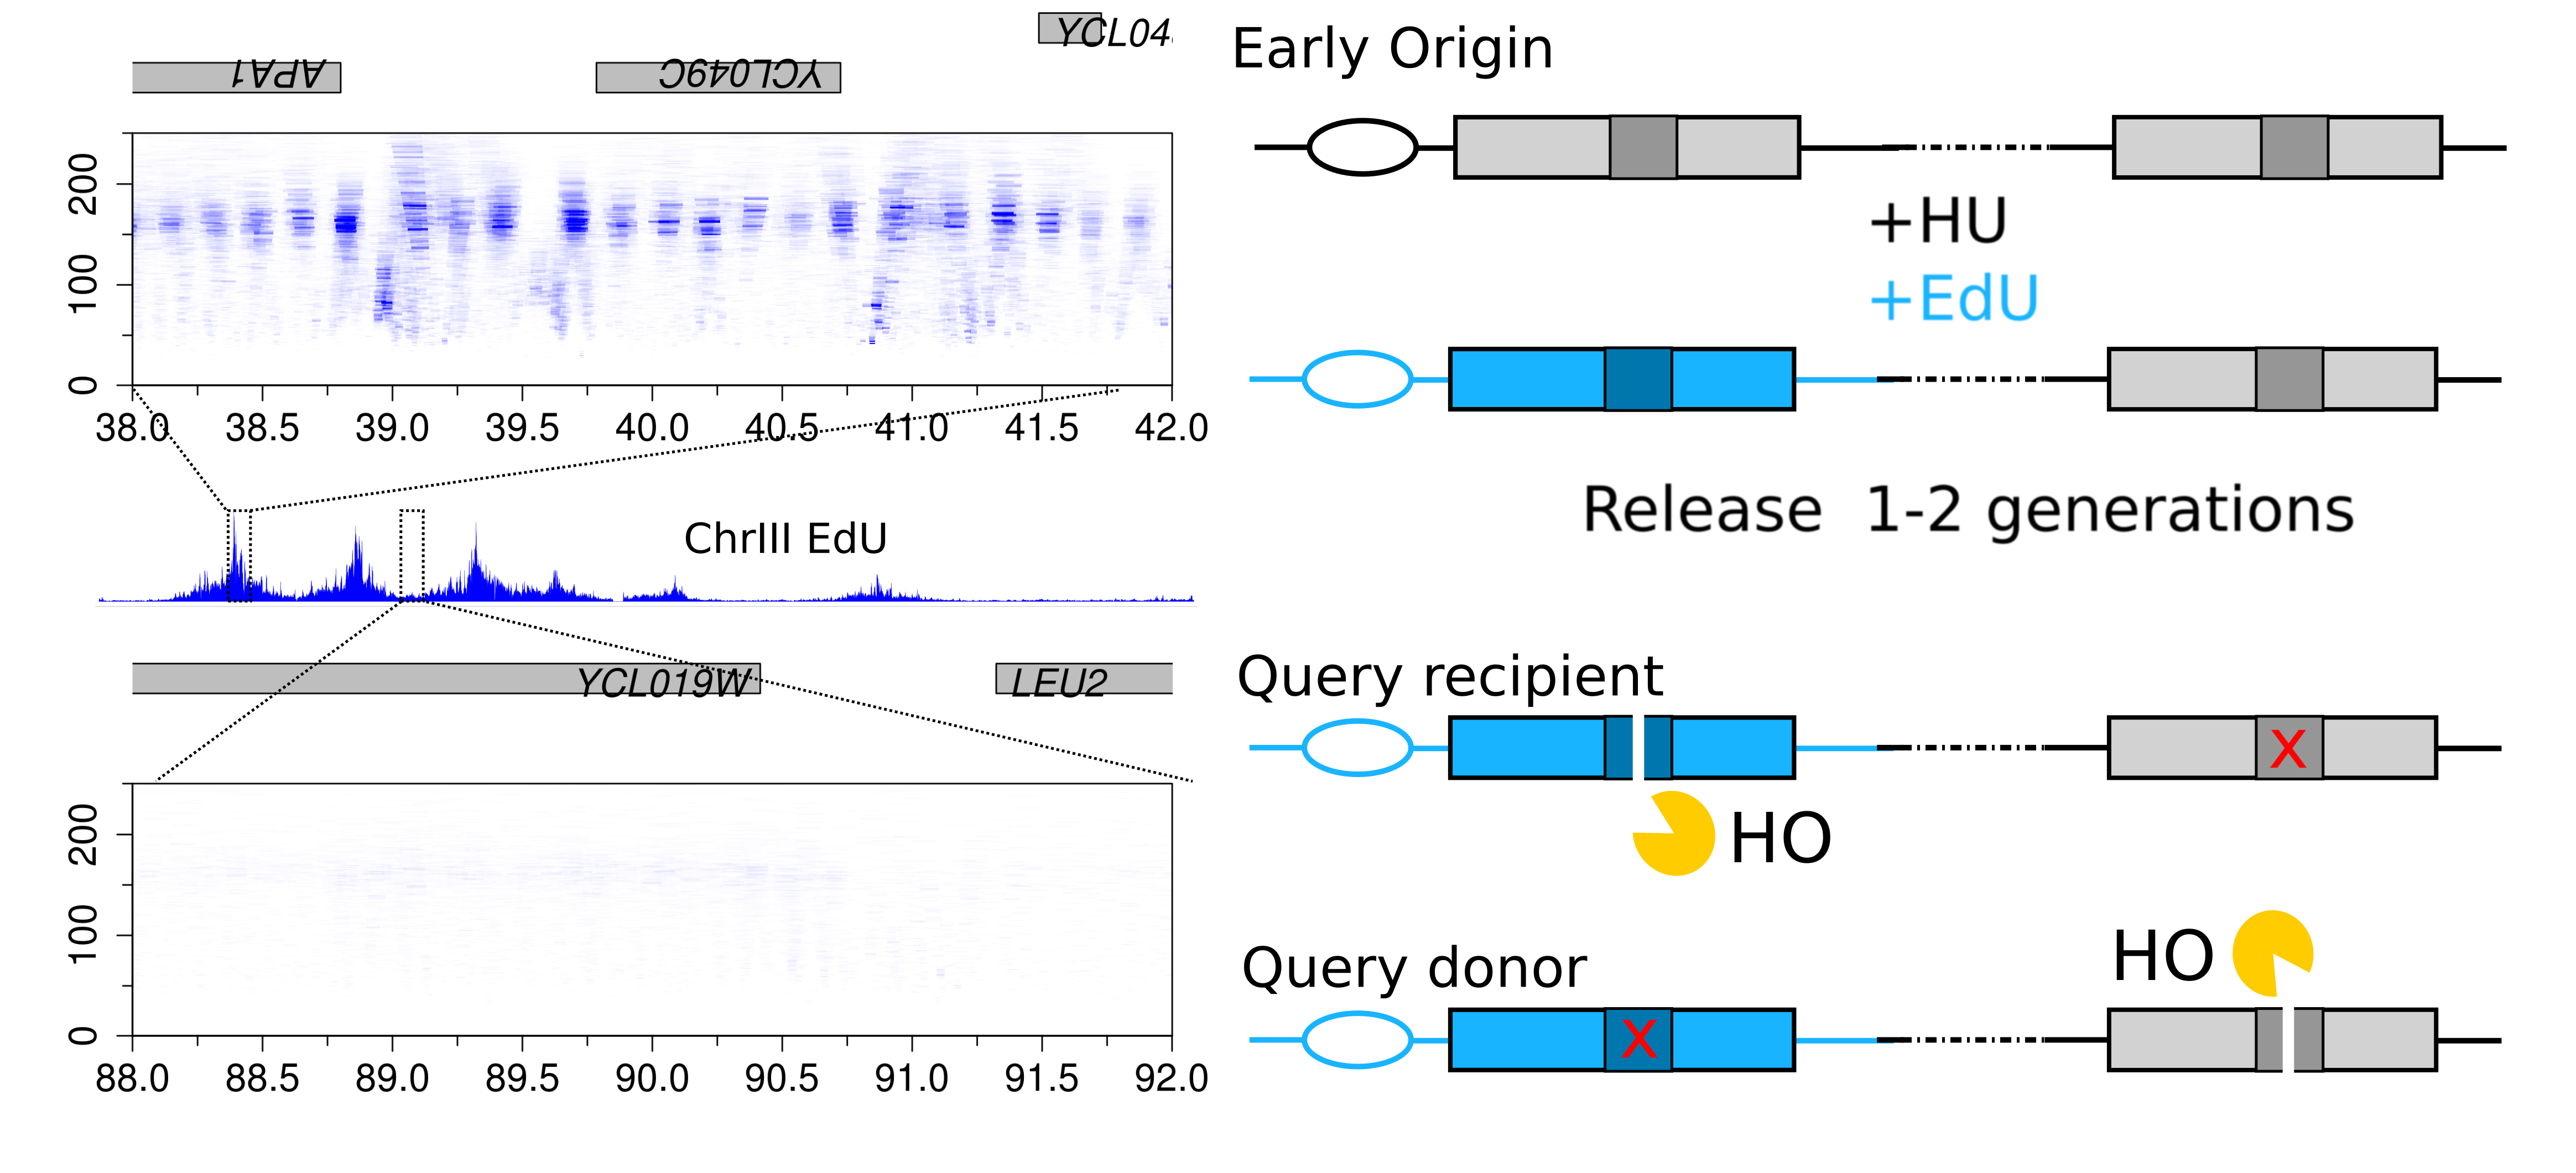
\includegraphics[width=3.65in]{r35_figures/edu_schematic_27.png}
\end{center}
\vspace{7mm}
\caption{Differentiating donor from recipient chromatin.  \textbf{Left}. Proof of principle EdU labeling early origin proximal chromatin structure.  \textbf{Right}.  Schematic for labeling either donor or recipient (damaged) DNA. A point mutation (red X) disrupts the HO cute site.}%
\end{floatingfigure}


%Importantly, both copies contain either an intact ectopic HO-endocuclease site or a 1 bp indel resistant to cleavage by HO-endonuclease.  Thus, we can induce a break in either the endogenous \texit{PHO5} locus or the identical \texit{ARS214} proximal copy which will enable us to specifically track the temporal progression of chromatin changes on either the donor or the break template.  Together these experiments will provide a nucleotide resolution view of the temporal kinetics of chromatin re-establishement and will likely provide critical insights into epigenetic state is preserved or lost following a DNA damage.

%siupstream of the \textit{PHO5} locus 

%We have engineered a yeast strain with an ectopic HO-endonuclease site upstream of \textit{PHO5} on chromosome II and ~4.5kb homologous donor sequence (containing a single 1bp indel resistant to cleavage by HO-endonuclease) that has been integrated adjacent to an early origin (\textit{ARS214} on the same chromosome.  

%Chromatin at the homologous donor template will be specifically labeled with EdU in the presence of HU and then released back into the cell cycle for at least one generation prior to generating the DSB.  Total chromatin will be digested with MNase to generate GCOPs. EdU specific GCOPs will be enriched by click chemistry-mediated biotinylation and streptavidin capture. We expect to identify donor specific perturbations of chromatin structure that are required to facilitate strand invasion and repair.

%nhej in G1 arrested cells. G2 will have donor



%In collaboration with Jim Haber (Brandeis; see letter of support) we have begun to elucidate the chromatin changes that occur 

%In order to repair a double strand break through HR, a search for a homologous donor sequence must be efficiently conducted across the genome.  Recent \invitro single molecule experiments with rad51 or recA pre-synaptic nucleoprotein filaments have begun to elucidate the mechanics of homology search on naked donor template DNA\cite{Renkawitz2014}.  However, a major question remains -- how is homology search conducted \invivo by the rad51 presynaptic filament in the context of chromatin? Recombination induced gene-conversion experiments have clearly demonstrated a dependence on chromatin remodelers such as INO80\cite{Tsukuda2009,Horigome2014}.  A major challenge to addressing this question using genome-wide approaches is the inability to readily distinguish homologous donor sequences from the sequence-identical damaged template DNA.   We propose to discriminate between the donor and break template by specifically labeling donor template with the nucleoside analogue, EdU ({\color{dukeblue}\textbf{Figure 6}}).   We and others have previously demonstrated that it is possible to specifically label only those sequences proximal ($<$15 kb) to early replicating origins, by releasing cells from a G1 alpha factor arrest into hydroxyurea (HU) in the presence of BrdU or EdU\citep{Peace2016-rb,Belsky2015-li}.  Importantly, these cells can be released back into the cell cycle for several generations and will retain the early origin-specific labeling albeit at diluted levels.  We have engineered a yeast strain with an ectopic HO-endonuclease site upstream of \textit{PHO5} on chromosome II and ~4.5kb homologous donor sequence (containing a single 1bp indel resistant to cleavage by HO-endonuclease) that has been integrated adjacent to an early (\textit{ARS214} or \textit{ARS305}) on the same or different chromosome.  Chromatin at the homologous donor template will be specifically labeled with EdU in the presence of HU and then released back into the cell cycle for at least one generation prior to generating the DSB.  Total chromatin will be digested with MNase to generate GCOPs.  EdU specific GCOPs will be enriched by click chemistry-mediated biotinylation and streptavidin capture. We expect to identify donor specific perturbations of chromatin structure that are required to facilitate strand invasion and repair.  Finally, we should be able to delay or repress specific remodeling events by the depletion or sequestration of key ATP-dependent chromatin remodelers (\eg Ino80).

%\newpage

\sheading{Transcription}
A major challenge in the post-genomic era is to understand how the information encoded in a static DNA sequence is capable of dynamic and regulated cell type specific patterns of gene expression. We are working in collaboration  with Alex Hartemink (PI) and Greg Crawford to develop predictive models of genome-wide transcript production from genome-wide chromatin occupancy data (R01 GM118551). %({\color{dukeblue}\textbf{Figure 7}}). 
Specifically, robust statistical models are being developed and validated for predicting gene expression by simultaneously monitoring real-time chromatin occupancy and dynamic transcription rates as synchronized yeast cells progress through the cell cycle\citep{Orlando2008-jq}.  Importantly, the statistical framework and quantitative tools developed for this project will be also be applicable to modeling the temporal dynamics of chromatin changes that occur during DNA replication and repair.
%\begin{floatingfigure}[l]{2.5in}
%\vspace{-5mm}
%\begin{center}
%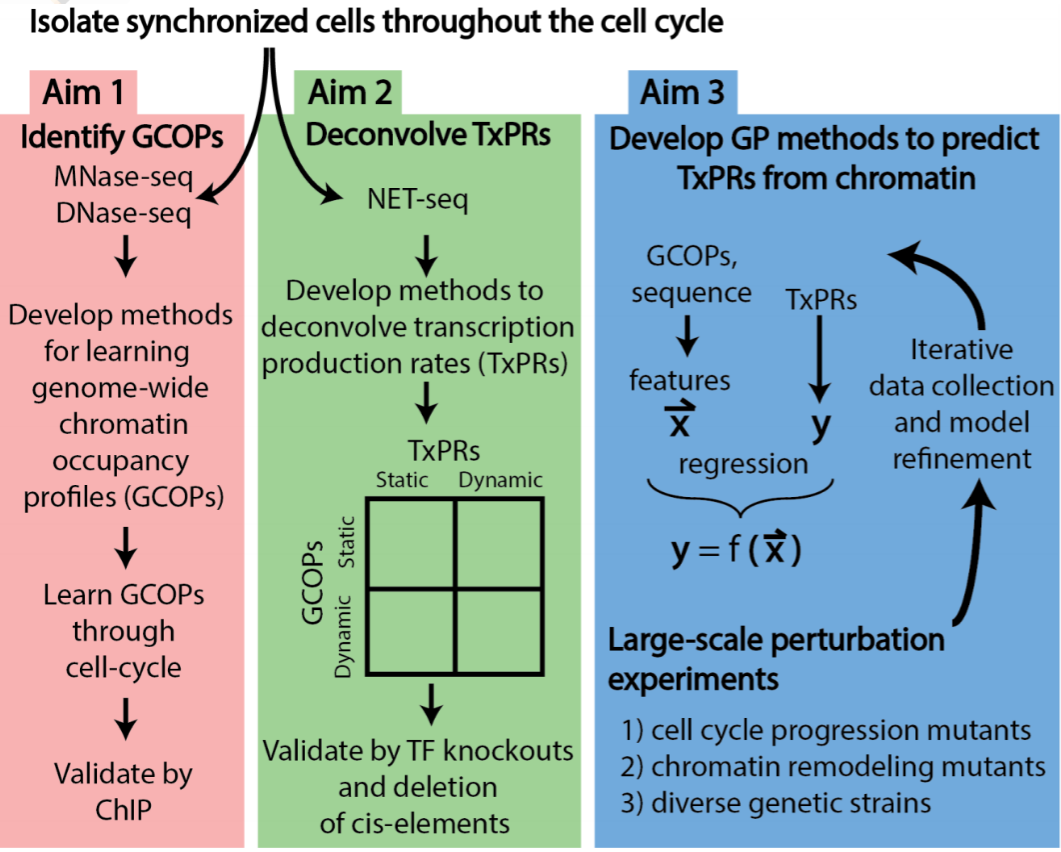
\includegraphics[width=2.5in]{r35_figures/gcop_strategy.png}
%\end{center}
%\vspace{2mm}
%\caption{Schematic describing the approach and methodologies to develop predictive models of cell cycle regulated gene expression from chromatin occupancy data. }%
%\end{floatingfigure}

My research program has benefited from the long standing collaboration we have had with the Hartemink group\citep{MacAlpine2010-ju,Belsky2015-li}.  Contributing to the success of the collaboration is the physical proximity of our research space in the Levine Science Research Center and mutual interest in cell cycle, DNA replication and chromatin structure.  We fully expect this productive collaboration to continue into the foreseeable future. 

\pagebreak
\bibliography{paperpile}


%Expected findings:
%-no change suggests homology search supports the model of querying donor strands while associated with histones on the outside
%- we will likely see a change since haber saw something in a locus adjacent to MATa (basically saw nucleosome depletion)
%Rad51 dependent changes suggest changes specific to homology search and not dsb
%Search from inside out or proximal edge? length of homology needed? where does search start.
%cis vs trans donor/break
%Extent of chromatin remodeling
%Impact of in80

%Recipriocal experiment -- Specially label cut site at ARS214 and/or ARS305 to rule out broader chromatin effects. but also query the chromatin changes that occur following repair of the break. how is broken chromatin reestablished.

%Epigenetic scar at donor or break

%Alternative approach -- also possible to do ChIP-seq for specific factors (eg. rad51) on EdU labeled chromatin. ORGANIC-ChIP + EdU (this is getting complicated but cool)




%they are thought to promote chromatin assembly and dissasembly at the replication fork.  

%their role at o

%MCM complex histone H3 interaction which 


%The Mcm2 subunit has been shown to directly interact with histone H3 presumably to faciliate chromatin disassembly and assembly ahead of the replication fork.  Work from our laboratory and rhind laboratory suggest that Mcm also appears to be in complex with nucleosome at the origin during G1.  




%We will test the impact of the mcm mutant on complex formation -- unlikey to be an intitation defect.  We will also take a proteomic approach to identify possible 



%Work in the Rhind laboratory has shown that chromatin immunoprecipitation of the MCM complex from MNase treated chromatin results in the recovery of nucleosomal sized DNA fragments\cite{}. 

%stochastic transcription termination.  

%Mcm2-7 has been previously shown to interact with histone H3 via ...  Although, this interaction is thought to mediate chromatin assembly via asf1, it may also be necessary for the observed Mcm2-7 nucleosome interaction at the origin.  We will test this hypothesis by performing ChIp-seq on mutant Mcm2-7. If the amino acid is required for nucleosome interaction, we will expect to lose the mcm-27+nucleosome chip-signal.  Could be shaped by nearby 3' transcription. To avoid torriosional consequences. knock out the promoter.



%We will 

%epigenetic angle -- specific modifications -- proteomic approach

%histone interaction domain?





%We will use a 

%Specific questions we hope to address include 

%Although


%Put another way -- at origin, we find the Mcm2-7 complex associated with either the up or down stream nucleosome.  Similar results were also identified by Nick Rhind and colleagues.  What is the molecular basis for this symmetry and nucleosome association? and how does it impact origin efficiency and timing. 



%How to identify factors that limit 1 mcm double hexamer per origin.  candidate approach.  multiple mcm loading -- stepwise during double hexamer loading...

%histone modifications?  topological constraints? why do both nucleosomes not become loaded?

%proteomic approach?  transcription and supercoiling?  examine netseq and supercoiling parameters during displacement via transcription?  Does transcription shape the effect? h3.3





%\sssheading{level 3} What does this look like. in the greater context.
%mcm loading -- asymmmetry. proteomic apprroach 

%factors that direct -- txp?

%Tie into in vitro experiments with Steve Bell.  We 
%The MacAlpine and Hartemink groups have had a long standing collaboration 

%This work will not only reveal how changes in chromatin occupancy are related to gene expression

%The proposed research will result in (i) efficient new methods for producing quantitative GCOPs that will be applicable in any organism with a sequenced genome; (ii) GCOPs from budding yeast as they progress through the cell cycle, revealing for the first time in any organism how genome-wide chromatin occupancy changes over the course of the cell cycle; (iii) characterization of how genome-wide chromatin changes are linked to changes in TxPRs, not only in wild-type yeast, but also under a wide range of genetic and genomic perturbations; and (iv) models learned from all these data that can predict TxPRs on the basis of chromatin occupancy, providing mechanistic insight into how the cell-cycle–regulated transcription program is influenced by its changing chromatin state. The DNA sequence of the genome is static, yet the dynamics in chromatin state and transcription rates can  Importantly, this project will allow us to look into the black box of chromatin Cell cycle -- This work will overtake our commitment with Hartemink laboratory to characterize big picture question of cell cycle regulation look inside black box. 



%Though the genome’s sequence is essentially fixed, its state may be constantly changing inside a cell. Two aspects of this changing state are the specific arrangement of myriad protein complexes along the genome in the form of chromatin, and the current rate of transcript production for each gene. A fundamental research objective is to understand the relationship between these two, and in particular, how transcript production rates (TxPRs) are influenced by genome-wide chromatin state. The goal of this proposal is to develop models that are capable of predicting a cell’s genome-wide transcription state from knowledge of its genome-wide chromatin state. To build such models requires simultaneously profiling a cell’s genome-wide chromatin state and transcription state at different times or under different conditions: Observing how the two change together, particularly in the context of directed perturbation, provides the statistical leverage needed to build predictive models that can provide causal insight. In this proposal, models will be developed and validated by monitoring chromatin and transcription in budding yeast as they progress through the cell cycle, a temporal series of highly regulated events controlling cell proliferation, aberrations of which can lead to cancer. Owing to the complexity of this challenge, yeast is used as a starting point because of its compact genome and genetic tractability, but we anticipate our methods will also be applicable in more complex organisms, including human. One major obstacle is that state-of-the-art chromatin immunoprecipitation (ChIP) methods for assaying chromatin state require a separate experiment not only for each time point and experimental condition, but also for each of the 100s–1000s of types of proteins binding along the genome. To overcome this hurdle, this proposal describes a novel method for efficiently learning quantitative genome-wide chromatin occupancy profiles (GCOPs) using nuclease-digested chromatin at single-base resolution. The proposed method enables the comprehensive determination of quantitative chromatin occupancy of transcription factors, nucleosomes, and other DNA-binding factors across the entire genome without requiring a separate experiment for each. Producing GCOPs in conjunction with high resolution measurements of TxPRs will allow the development of sophisticated, mechanistically interpretable models that predict transcript production rates as a function of chromatin state.

%The proposed research will result in (i) efficient new methods for producing quantitative GCOPs that will be applicable in any organism with a sequenced genome; (ii) GCOPs from budding yeast as they progress through the cell cycle, revealing for the first time in any organism how genome-wide chromatin occupancy changes over the course of the cell cycle; (iii) characterization of how genome-wide chromatin changes are linked to changes in TxPRs, not only in wild-type yeast, but also under a wide range of genetic and genomic perturbations; and (iv) models learned from all these data that can predict TxPRs on the basis of chromatin occupancy, providing mechanistic insight into how the cell-cycle–regulated transcription program is influenced by its changing chromatin state. The DNA sequence of the genome is static, yet the dynamics in chromatin state and transcription rates can  Importnatly, this project will allow us to look into the black box of chromatin Cell cycle -- This work will overtake our commitment with Hartemink laboratory to characterize big picture question of cell cycle regulation look inside black box. 
\section*{Resource Sharing Plans}
We are committed to openly share the data and resources developed in the course of this project.  Genomic data will be disseminated in publicly available repositories (\eg NCBI GEO).  Software developed in the project will be shared using GitHub.  Protocols will be distributed via Protocol Exchange and the investigator's web site.  All cell lines, strains and plasmid constructs will be provided upon request.
\end{document}